\documentclass[a4paper, 12pt]{extreport}
\usepackage[utf8]{inputenc}
\usepackage[english,russian]{babel}
\usepackage{amssymb,amsfonts,amsmath,mathtext,cite,enumerate,float}
\usepackage{pgfplots}
\usepackage{graphicx}
\usepackage[inkscapeformat=png]{svg}
\usepackage{tocloft}
\usepackage{listings}
\usepackage{caption}
\usepackage{tempora}
\usepackage{titlesec}
\usepackage{setspace}
\usepackage{geometry}
\usepackage{indentfirst}
\usepackage{pdfpages}
\usepackage{enumerate,letltxmacro}
\usepackage{threeparttable}
\usepackage{hyperref}
\usepackage{flafter}
\usepackage{enumitem}
\usepackage{multirow}
\usepackage{mathtools}
\usepackage{longtable}
\usepackage[figure,table]{totalcount}
\usepackage{lastpage}

\lstdefinestyle{python}{
	language={Python},
	basicstyle=\footnotesize\ttfamily,
	numbers=left,
	frame=single,
	tabsize=4,	
	breaklines=true
}

\setlist{nosep}
\hypersetup{pdfborder=0 0 0}

\newcommand{\ssr}[1]{\begin{center}\LARGE\bfseries{#1}\end{center} \addcontentsline{toc}{chapter}{#1}  }

\makeatletter
\renewcommand\LARGE{\@setfontsize\LARGE{22pt}{20}}
\renewcommand\Large{\@setfontsize\Large{20pt}{20}}
\renewcommand\large{\@setfontsize\large{16pt}{20}}
\makeatother

\RequirePackage{titlesec}
\titleformat{\chapter}[block]{\hspace{\parindent}\large\bfseries}{\thechapter}{0.5em}{\large\bfseries\raggedright}
\titleformat{name=\chapter,numberless}[block]{\hspace{\parindent}}{}{0pt}{\large\bfseries\centering}
\titleformat{\section}[block]{\hspace{\parindent}\large\bfseries}{\thesection}{0.5em}{\large\bfseries\raggedright}
\titleformat{\subsection}[block]{\hspace{\parindent}\large\bfseries}{\thesubsection}{0.5em}{\large\bfseries\raggedright}
\titleformat{\subsubsection}[block]{\hspace{\parindent}\large\bfseries}{\thesubsection}{0.5em}{\large\bfseries\raggedright}
\titlespacing{\chapter}{12.5mm}{-22pt}{10pt}
\titlespacing{\section}{12.5mm}{10pt}{10pt}
\titlespacing{\subsection}{12.5mm}{10pt}{10pt}
\titlespacing{\subsubsection}{12.5mm}{10pt}{10pt}

\makeatletter
\renewcommand{\@biblabel}[1]{#1.}
\makeatother

\geometry{left=30mm}
\geometry{right=10mm}
\geometry{top=20mm}
\geometry{bottom=20mm}

\onehalfspacing

\renewcommand{\theenumi}{\arabic{enumi}}
\renewcommand{\labelenumi}{\arabic{enumi}\text{)}}
\renewcommand{\theenumii}{.\arabic{enumii}}
\renewcommand{\labelenumii}{\asbuk{enumii}\text{)}}
\renewcommand{\theenumiii}{.\arabic{enumiii}}
\renewcommand{\labelenumiii}{\arabic{enumi}.\arabic{enumii}.\arabic{enumiii}.}

\renewcommand{\cftchapleader}{\cftdotfill{\cftdotsep}}

\addto\captionsrussian{\renewcommand{\figurename}{Рисунок}}
\DeclareCaptionLabelSeparator{dash}{~---~}
\captionsetup{labelsep=dash}

\captionsetup[figure]{justification=centering,labelsep=dash}
\captionsetup[table]{labelsep=dash,justification=raggedright,singlelinecheck=off}
\captionsetup[lstlisting]{labelsep=dash,justification=raggedright,singlelinecheck=off}

\newcommand{\floor}[1]{\lfloor #1 \rfloor}

\pgfplotsset{width=0.85\linewidth, height=0.5\columnwidth}

\linespread{1.3}

\parindent=1.25cm

\def\labelitemi{---}
\setlist[itemize]{leftmargin=1.25cm, itemindent=0.65cm}
\setlist[enumerate]{leftmargin=1.25cm, itemindent=0.55cm}

\newcommand{\specialcell}[2][c]{\begin{tabular}[#1]{@{}c@{}}#2\end{tabular}}
\frenchspacing


\begin{document}
\begin{titlepage}
	\newgeometry{pdftex, left=2cm, right=2cm, top=2.5cm, bottom=2.5cm}
	\fontsize{12pt}{12pt}\selectfont
	\noindent\begin{tabular}{|c|c|}	\hline
	\noindent\begin{minipage}{0.15\textwidth}
		
\includegraphics[width=\linewidth]{tools/logo.png}
	\end{minipage} &
	\noindent\begin{minipage}{0.85\textwidth}\centering
		\textbf{\newline Министерство науки и высшего образования Российской Федерации}\\
		\textbf{Федеральное государственное бюджетное образовательное учреждение высшего образования}\\
		\textbf{«Московский государственный технический университет имени Н.Э.~Баумана}\\
		\textbf{(национальный исследовательский университет)»}\\
		\textbf{(МГТУ им. Н.Э.~Баумана)}
	\end{minipage} \\
	\hline	\end{tabular}\newline\newline\newline
	\noindent ФАКУЛЬТЕТ \underline{«Информатика и системы управления»} \newline\newline
	\noindent КАФЕДРА \underline{«Программное обеспечение ЭВМ и информационные технологии»}\newline\newline\newline\newline\newline\newline

	\noindent\begin{minipage}{1.0\textwidth}\centering
		\Large\textbf{       Лабораторная работа №7}
		\end{minipage}
		
	\noindent\begin{minipage}{1.0\textwidth}\centering
		\textbf{\newline}	
		\end{minipage}

	\noindent\begin{minipage}{1.0\textwidth}\centering
		\Large\textbf{по дисциплине «Анализ алгоритмов»}	
		\end{minipage}
		
	\noindent\begin{minipage}{1.0\textwidth}\centering
		\Large\textbf{\newline\newline\newline\newline}	
		\end{minipage}
		
	\noindent\textbf{Тема} \underline{Графовые модели}\newline\newline
	\textbf{Студент} \underline{Тузов Даниил Александрович}\newline\newline
	\textbf{Группа} \underline{ИУ7-52Б}\newline\newline
	\textbf{Преподаватель} \underline{Волкова Лилия Леонидовна}
	
	\begin{center}
		\vfill
		Москва, \the\year~г.
	\end{center}
	\restoregeometry
	\clearpage
\end{titlepage}



\setlength{\cftbeforetoctitleskip}{-4mm}
\renewcommand{\contentsname}{\makebox[\textwidth][c]{\largeСОДЕРЖАНИЕ}}
\tableofcontents
\setcounter{page}{2}

\clearpage\ssr{ВВЕДЕНИЕ}

В 7 лабораторной работе рассматриваются графовые модели.

Целью работы является описание 4 графовых моделей на примере выбранного фрагмента кода. Для достижения поставленной 
цели необходимо решить следующие задачи:
\begin{itemize}
	\item[---] выбрать фрагмент кода, для которого будут строиться графовые модели;
	\item[---] построить информационный граф;
	\item[---] построить информационную историю;
	\item[---] построить граф управления;
	\item[---] построить операционную историю.
\end{itemize}

\chapter{Исходный код, выбранного алгоритма}

Были поставлены следующие требования к фрагменту кода:
\begin{itemize}
	\item[---] 15 или более значащих строк кода (не пробелы, не комментарии, не фигурные скобки);
	\item[---] в коде есть хотя бы 2 цикла, среди которых один вложен в другой.
\end{itemize}

По этой причине был выбран код основной функции муравьиного алгоритма. Код представлен в листинге~\ref{lst:ant}.

\begin{lstlisting}[style=python, label=lst:ant,caption=Муравьиный алгоритм]
def ant_alg(mat, alpha, ro, t_max):
    n, q = len(mat), calc_q(mat)
    pheromone = init_pheromone(n)
    attract = init_attract(mat)
    min_path_len = -1
    best_path = list()
    for t in range(t_max):
        memory = init_memory(n)
        for ant in range(n):
            while len(memory[ant]) != n:
                p = calc_p(pheromone, attract, memory[ant], n, alpha)
                memory[ant].append(calc_next(p))
            path_len = calc_length(mat, memory[ant])
            if min_path_len == -1 or min_path_len > path_len:
                min_path_len = path_len
                best_path = memory[ant]
        pheromone = update_pheromone(mat, memory, pheromone, q, ro)
    for i in range(len(best_path)):
        best_path[i] += 1
    return best_path, min_path_len
\end{lstlisting}

\chapter{Информационный граф}

Информационный граф (ИГ) --- это такая модель программы, в которой вершины --- это команды, операторы или строки кода, а дуги --- информационное отношение.

Информационное отношение --- это отношение по передаче данных.

Информационный граф для муравьиного алгоритма представлен на рисунке~\ref{graph-inf}.

\begin{figure}[h]
	\centering
	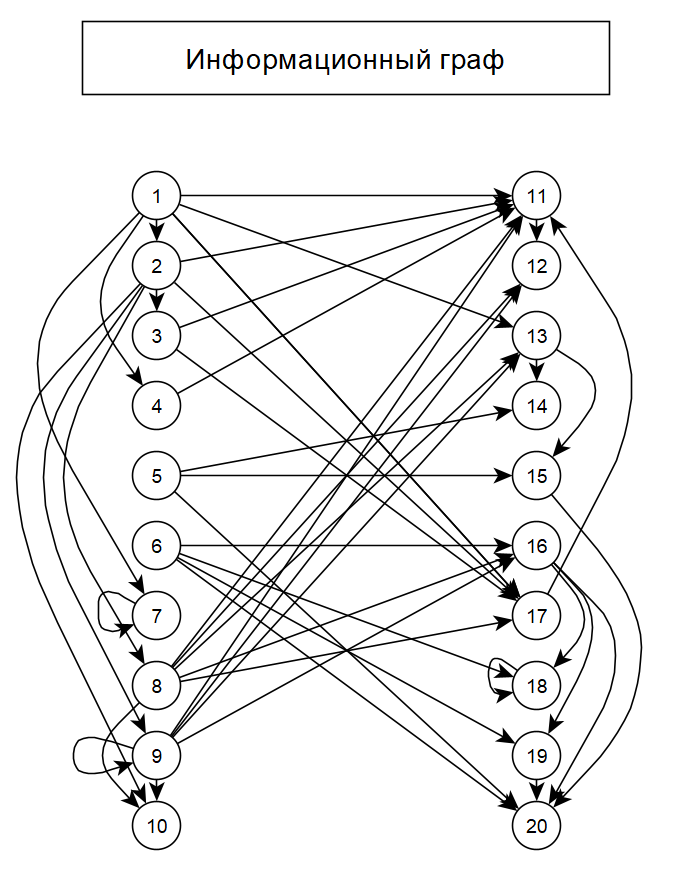
\includegraphics[scale=1]{tools/graph-inf.png}
	\caption{Информационный граф}
	\label{graph-inf}
\end{figure}

\chapter{Граф управления}

Граф управления (ГУ) --- это такая модель программы, в которой вершины --- это команды, операторы или строки кода, а дуги 
--- операционное отношение.

Операционное отношение --- это отношение по передаче управления.

Граф управления для муравьиного алгоритма представлен на рисунке~\ref{graph-control}.

\begin{figure}[h]
	\centering
	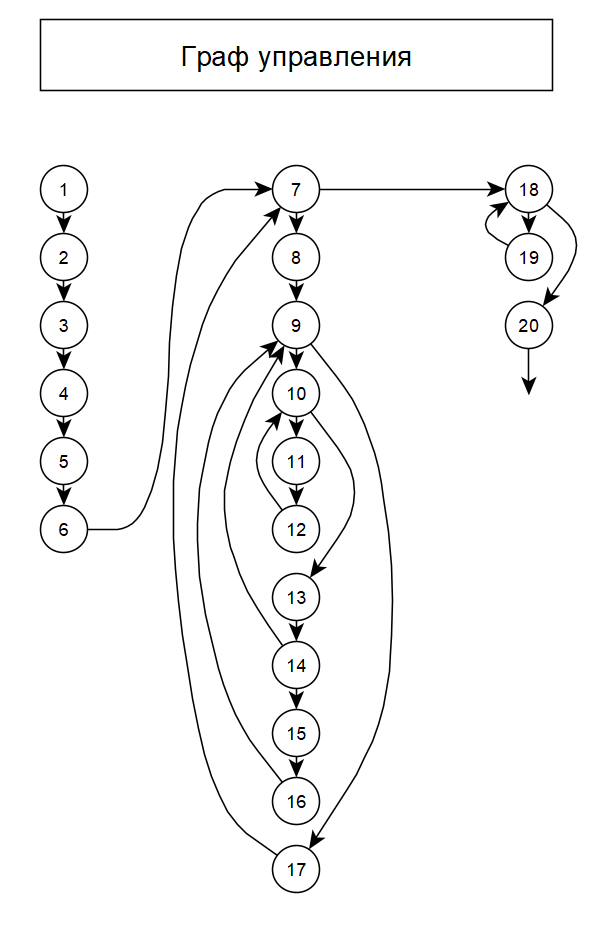
\includegraphics[scale=0.9]{tools/graph-control.png}
	\caption{Граф управления}
	\label{graph-control}
\end{figure}

\chapter{Информационная история}

Информационная история при анализе алгоритма --- это информационное отношение между вершинами графа, отражающее, 
как одна вершина использует в качестве аргумента значение, полученное в другой.

Информационная история для муравьиного алгоритма представлен на рисунке~\ref{graph-inf-hist}.

\begin{figure}[h]
	\centering
	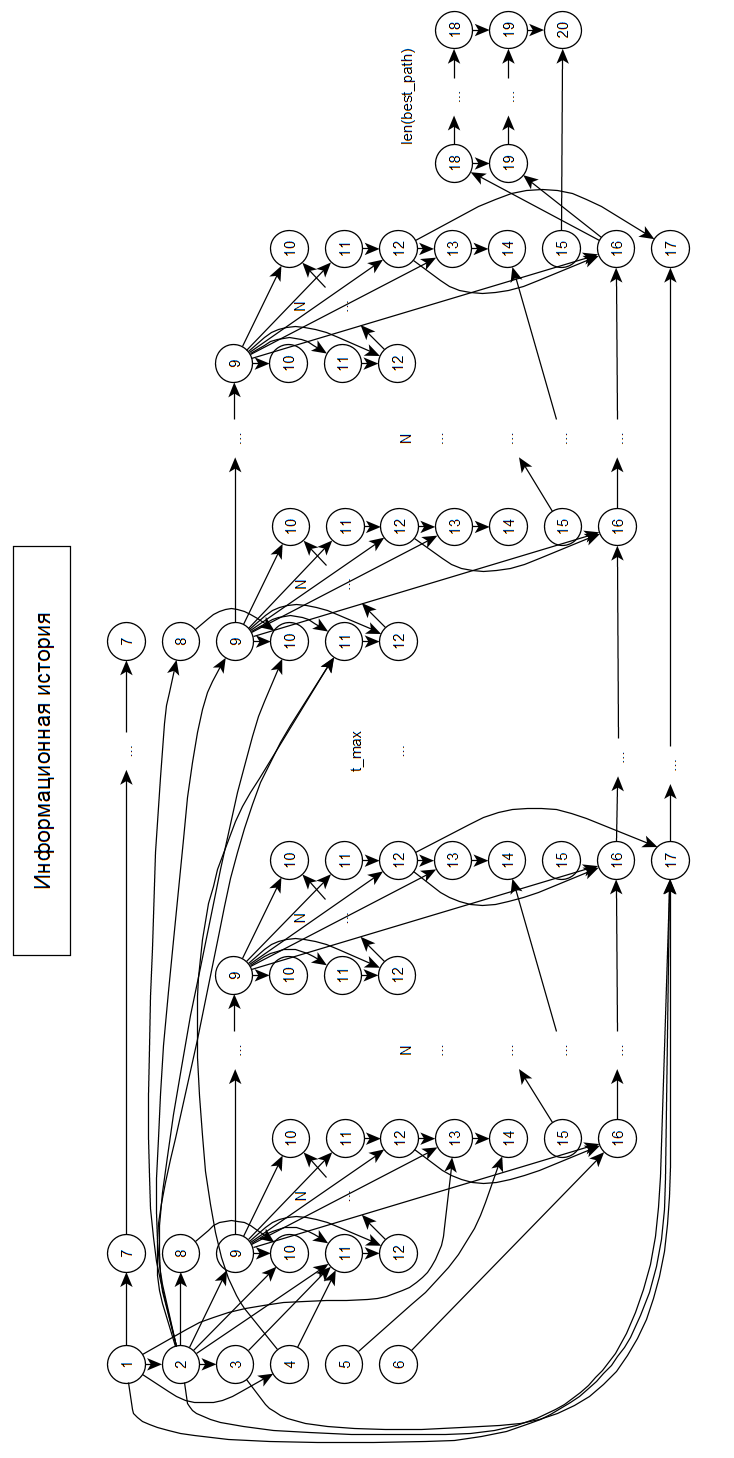
\includegraphics[scale=0.6]{tools/graph-inf-hist.png}
	\caption{Информационная история}
	\label{graph-inf-hist}
\end{figure}


\chapter{Операционная история}

Операционная история --- это операционное отношение между вершинами, означающее, что одна вершина может быть 
выполнена сразу после другой. Является строго линейной.

Операционная история для муравьиного алгоритма представлен на рисунке~\ref{graph-op-hist}.

\begin{figure}[h]
	\centering
	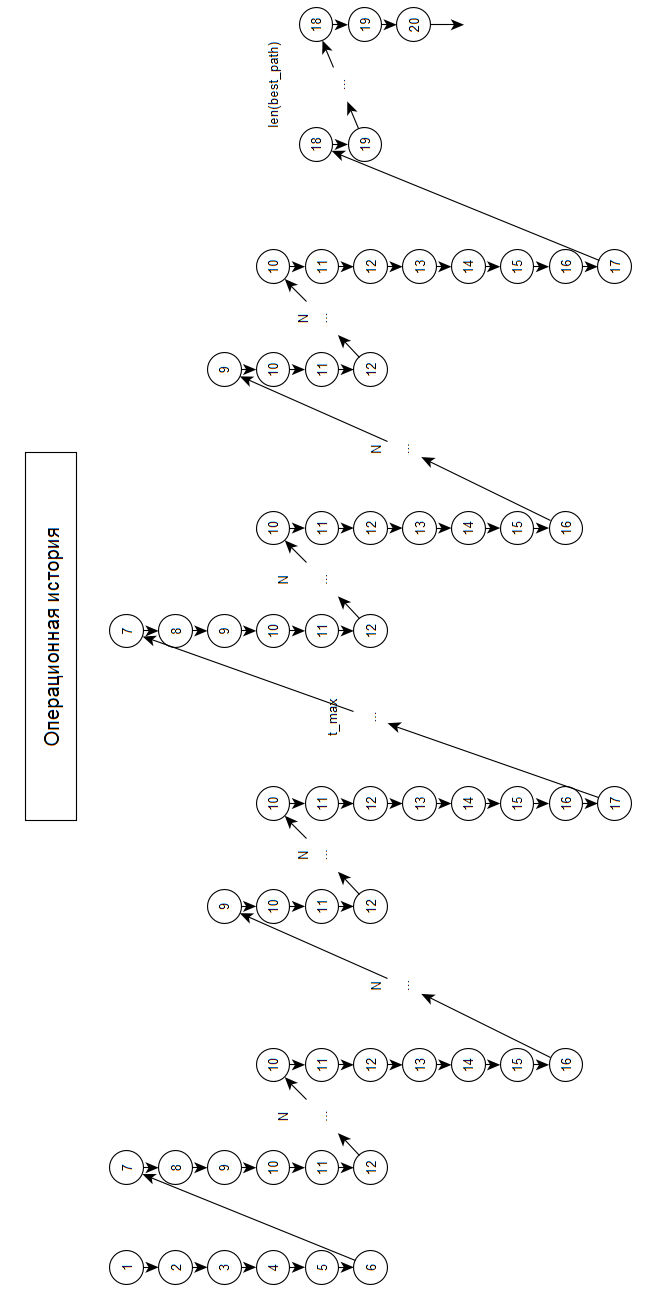
\includegraphics[scale=0.6]{tools/graph-op-hist.png}
	\caption{Операционная история}
	\label{graph-op-hist}
\end{figure}

\clearpage\ssr{ЗАКЛЮЧЕНИЕ}

В ходе выполнения лабораторной работы поставленная цель была достигнута. Были решены все задачи:
\begin{itemize}
	\item[---] реализована основная функция муравьиного алгоритма;
	\item[---] построен информационный граф;
	\item[---] построена информационную историю;
	\item[---] построен граф управления;
	\item[---] построена операционную историю.
\end{itemize}

\end{document}